\chapter{Reti di Flusso}
Una rete è un grafo pesato a cui nodi e archi sono associati dei valori detti \textbf{pesi}. In una rete, gli archi sono dei canali dentro cui vi fluiscono dei beni che possono essere rappresentate per mezzo di grandezze \textbf{discrete} o \textbf{continue} e possono rappresentare dei valori \textbf{assoluti} o dei valori \textbf{relativi} come, ad esempio, per unità di tempo. In questo contesto i pesi degli archi rappresentano la \textbf{capacità e dei costi} mentre i pesi sui nodi possono rappresentare la quantità di beni che entrano in quei nodi o che ne escono.\\
Formalmente una rete di flusso è definita come un grafo orientato $G = (V, E)$ senza cappi e tale che:
\begin{itemize}
    \item A ogni arco $(u, v) \in E$ è associato un valore non negativo, $c(u, v) \geq 0$, detto \textbf{capacità} dell'arco. Se l'arco $(u, v)$ non è presente in $E$ allora assumiamo che esso abbia capacità nulla, cioè $c(u, v) = 0$.
    
    \item Nella rete di flusso ci sono due vertici speciali: il vertice \textbf{sorgente}, indicato con il simbolo $s$, e il vertice \textbf{pozzo} (o \textbf{destinazione}), indicato con il simbolo $t$. \\
    I rimanenti vertici sono detti \textbf{vertici di transizione}.
    
    \item Ogni vertice giace su qualche cammino dalla sorgente al pozzo. Il grafo è quindi connesso e pertanto vale $|E| \geq |V| - 1$.
\end{itemize}
\begin{figure}[H]
    \centering
    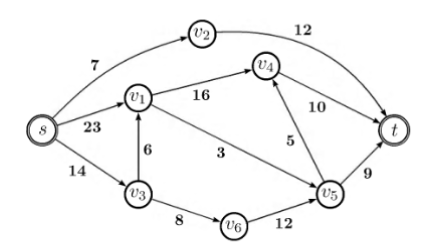
\includegraphics[width=0.5\linewidth]{Images/reti_di_flusso/esempio_di_rete.png}
\end{figure}

Data una rete $G=(V,E)$ con capacità $c: V \times V \to R_0^+$ un \textbf{flusso reale} in $G$ è una funzione $\varphi: V \times V \to R_0^+$ soddisfa i seguenti requisiti:
\begin{itemize}
    \item \textbf{Vincolo di Capacità:} per ogni arco $(u,v) \in V\times V$ si richiede che $\varphi(u,v) \leq c(u,v)$ che ci dice che non possiamo fare passare più risorse di quanta sia la capacità dell'arco.
    \item \textbf{Conservazione del flusso (legge di Kirchhoff):} Per tutti gli archi $u\in V - \{s,t\}$ si richiede che:
    \[\sum \varphi(u,v) \text{ \textbf{flusso uscente}} = \sum \varphi(v, u) \text{ \textbf{flusso entrante}}\]
    Cioè, tutto quello che entra in un nodo intermedio deve anche uscire. Questa regola vale, naturalmente, per tutti i nodi tranne che per la sorgente e la destinazione.
\end{itemize}
Chiameremo \textbf{flusso reale} la quantità $\varphi(u,v)$ lungo l'arco (u, v).
Definiamo il \textbf{Valore del flusso reale come}:
\[|\varphi| = \sum_{v \in V} \varphi(s, v) - \sum_{v \in V} \varphi(v, s)\]
Il flusso totale della rete è calcolato guardando solo la Sorgente ($s$).
È la somma di tutto ciò che esce da $s$ meno tutto ciò che rientra in $s$.

\section{Problema del Massimo Flusso}
Definiamo il \textbf{problema del massimo flusso} in una rete di flusso come la determinazione di un flusso $\varphi$ in $G$ di valore massimo. Distinguiamo adesso due casi:
\begin{itemize}
    \item \textbf{Flusso Massimale}: Significa che, mantenendo fissi i percorsi che abbiamo già scelto, ciò che abbiamo ottenuto è il massimo che si può senza violare le regole.
    \item \textbf{Flusso Massimo}: È l'ottimo globale, cioè il flusso più alto che si può ottenere anche a costo di modificare scelte precedenti (\textbf{backtracking}). 
\end{itemize}
Per evitare il problema del backtracking, utilizziamo il concetto di \textbf{flusso netto}. 
Data una rete $G = (V, E)$ con capacità $c : E \to R^+_0$ e con un \textbf{flusso reale} 
$\varphi : V \times V \to R^+_0$, poniamo: 
\[f_\varphi(u, v) = \varphi(u, v) - \varphi(v, u) \quad \quad \forall (u,v) \in V \times V\]
\begin{figure}[H]
    \centering
    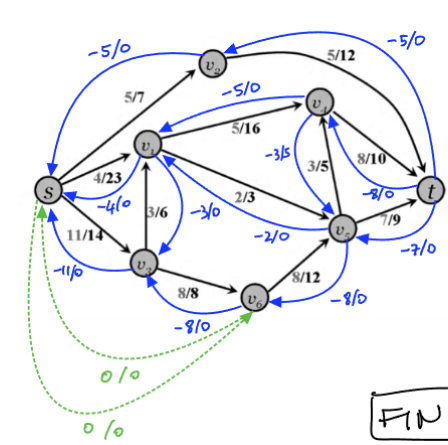
\includegraphics[width=0.5\linewidth]{Images/reti_di_flusso/esempio_flusso_netto.png}
\end{figure}
Nel grafico che vediamo, il flusso netto viene calcolato da un nodo al precedente. Da questo segue il fatto che il valore è negativo. Il flusso netto gode delle seguenti proprietà:
\begin{itemize}
    \item \textbf{Vincolo di capacità}: Il flusso netto da un vertice all'altro non può eccedere la corrispondente capacità:
    \[f_\varphi(u, v) \le c(u, v), \quad \text{per tutti gli } u, v \in V.\]
    \textit{Dimostrazione:}
    \[f_\varphi(u, v) = \varphi(u, v) - \varphi(v, u) \le \varphi(u, v) \le c(u, v)\]

    \item \textbf{Antisimmetria}:Il flusso netto in una direzione è l'opposto del flusso nella direzione inversa:
    \[f_\varphi(u, v) = -f_\varphi(v, u), \quad \text{per tutti gli } u, v \in V.\]
    Segue da ciò che il flusso netto da un vertice a sé stesso deve essere 0 poiché per ogni $u \in V$ abbiamo che $f_\varphi (u, u) = -f_\varphi(u, u)$ il che implica che $f_\varphi(u,u) = 0$ 
    \item \textbf{Conservazione del flusso}: Per ogni nodo intermedio (né sorgente né pozzo), la somma algebrica dei flussi netti uscenti è nulla:
    \[\sum_{v \in V} f_\varphi(u, v) = 0, \quad \text{per tutti gli } u \in V - \{s, t\}\]
    Cioè, il flusso netto uscente da $u$ è nullo poiché quello che entra è uguale a quello che esce. Allo stesso modo vale che:
    \[\sum_{v \in V} f_\varphi(v, u) = 0\]
    Cioè, il flusso netto entrante in un vertice di transizione deve essere obbligatoriamente nullo.
\end{itemize}

Sia $G = (V, E, c, s, t)$ una rete di flusso con funzione capacità $c$, sorgente $s$ e pozzo $t$ e sia $g : V \times V \to R$ una funzione che soddisfi:

\begin{itemize}
    \item Il vincolo di capacità (relativamente a $c$);
    \item La proprietà di antisimmetria;
    \item La legge di conservazione del flusso (relativamente a $s$ e a $t$).
\end{itemize}

Allora la funzione $\varphi_g : V \times V \to R^+_0$ definita da:

\[\varphi_g(u, v) = 
\begin{cases} 
    g(u, v) & \text{se } g(u, v) > 0 \\
    0 & \text{altrimenti}
\end{cases}
\]
È un \textbf{flusso reale} in $G = (V, E, c, s, t)$ che induce il flusso netto $g$, cioè:
\[g = f_{\varphi_g}\]
Dimostriamo che è possibile convertire $g$ in un flusso reale $\varphi_g$ :
\begin{itemize}
    \item \textbf{Vincolo di capacità per $\varphi_g$}:Per definizione abbiamo impostato:
    \[
        \varphi_g(u, v) = 
        \begin{cases} 
        g(u, v) & \text{se } g(u, v) > 0 \\
        0 & \text{altrimenti}
        \end{cases}
    \]
    Verifichiamo che rispetti la capacità $c(u,v)$:
    \begin{itemize}
        \item Se $g(u, v) > 0$, allora $\varphi_g(u, v) = g(u, v) \le c(u, v)$ (per ipotesi su $g$).
        \item Se $g(u, v) \le 0$, allora $\varphi_g(u, v) = 0 \le c(u, v)$ (poiché le capacità sono non negative).
    \end{itemize}
    E quindi, in ogni caso:
    \[\varphi_g(u, v) \le c(u, v)\]
    \item \textbf{Conservazione del Flusso per $\varphi_g$}: Sappiamo che per ogni coppia $u, v \in V$:
    \[\varphi_g(u, v) - \varphi_g(v, u) = g(u, v) \quad (*)\]
    Infatti, analizziamo i tre casi possibili per il valore di $g(u,v)$:
    \[\varphi_g(u, v) - \varphi_g(v, u) = 
    \begin{cases} 
        g(u, v) - 0 = g(u, v) & \text{se } g(u, v) > 0 \\
        \\
        0 - 0 = g(u, v) & \text{se } g(u, v) = 0 \\
        \\
        0 - g(v, u) = -g(v, u) = g(u, v) & \text{se } g(u, v) < 0
    \end{cases}
    \]\footnote{Ricordiamo che $g(u, v) = - g(v, u)$ dunque, se uno è positivo, l'altro è per forza negativo e, dunque, scatta lo zero.}
    Sia adesso $u \in V - \{s,t\}$, allora sappiamo che:
    \begin{align*}
        \sum_{v \in V} \varphi_g(u, v) - \sum_{v \in V} \varphi_g(v, u) &= \sum_{v \in V} \left( \varphi_g(u, v) - \varphi_g(v, u) \right) \\
        &= \sum_{v \in V} g(u, v) \quad \text{(Per la proprietà $(*)$)} \\
        &= 0 \quad \text{(Per ipotesi di conservazione su $g$)}
    \end{align*}
    Quindi il flusso reale si conserva:
    \[\sum_{v \in V} \varphi_g(u, v) = \sum_{v \in V} \varphi_g(v, u)\]
    Pertanto, $g$ è esattamente uguale al flusso netto indotto da $\varphi_g$.
\end{itemize}

Il \textbf{valore $|f|$} di un flusso $f$ è definito come:
\[|f| = \sum_{v\in V} f(s,v)\]
Se $f_\phi$ è un flusso netto indotto da un flusso reale $\varphi$, allora: 
\begin{align*}
    |f_\varphi| &= \sum_{v \in V} f_\varphi(s, v) \\
    &= \sum_{v \in V} (\varphi(s, v) - \varphi(v, s)) \\
    &= \sum_{v \in V} \varphi(s, v) - \sum_{v \in V} \varphi(v, s) \\
    &= |\varphi|.
\end{align*}

D'ora in poi indicheremo come \textbf{Problema del flusso massimo} il problema di determinare un \textbf{flusso netto $f$} in G di valore massimo da $s$ a $t$.
\begin{figure}[H]
    \centering
    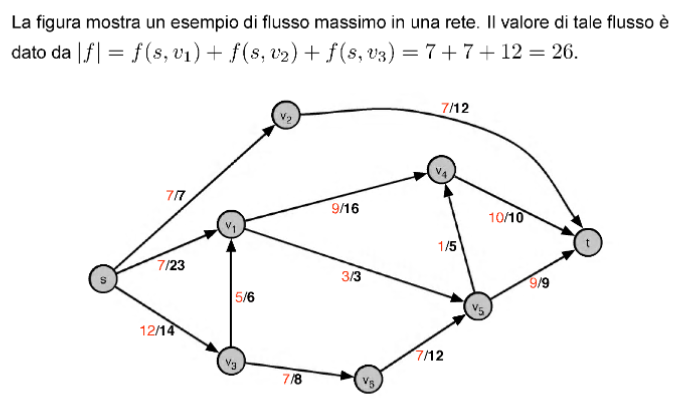
\includegraphics[width=0.75\linewidth]{Images/reti_di_flusso/flusso_massimo.png}
\end{figure}
Il problema di flusso massimo su una rete $G$ con più sorgenti $\{s_1, s_2, \dots, s_m\}$ e più pozzi $\{t_1, t_2, \dots, t_n\}$ può essere ricondotto a un problema di flusso massimo ordinario.
Questo viene fatto trasformando la rete $G$ in una rete di flusso ordinaria $G'$ con singola sorgente e singolo pozzo nel modo seguente:
\begin{itemize}
    \item si aggiunge una \textbf{super-sorgente} $s$ e un arco orientato $(s, s_i)$, per ogni $i = 1, \dots, m$, con capacità $c(s, s_i) = \infty$
    
    \item si aggiunge un \textbf{super-pozzo} $t$ e un arco orientato $(t_j, t)$, per ogni $j = 1, \dots, n$, con capacità $c(t_j, t) = \infty$
\end{itemize}
È facile verificare che ogni flusso nella rete $G'$ corrisponde a un flusso nella rete $G$.
\begin{figure}[H]
    \centering
    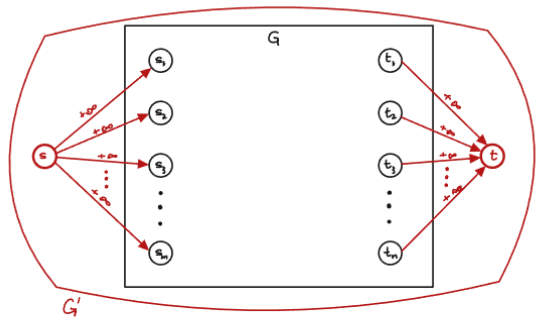
\includegraphics[width=0.5\linewidth]{Images/reti_di_flusso/pozzi_multipli.png}
\end{figure}


\subsection*{Lemma 1}
Siano $X$ e $Y$ due insiemi di vertici allora:
\[f(X, Y) = \sum_{x\in X}\sum_{y \in Y} f(x, y)\]

Sia $G = (V, E)$ una rete di flusso, e sia $f$ un flusso in $G$. Allora:

\begin{itemize}
    \item Per $X, Y \subseteq V$ si ha $f(X, Y) = -f(Y, X)$;
    
    \item Per $X \subseteq V$ si hanno $f(X, X) = 0$ e $f(\emptyset, X) = 0$;
    
    \item Per $X, Y, Z \subseteq V$, si hanno
    \begin{align*}
        f(X \cup Y, Z) &= f(X, Z) + f(Y, Z) - f(X \cap Y, Z) \quad \text{e} \\
        f(Z, X \cup Y) &= f(Z, X) + f(Z, Y) - f(Z, X \cap Y).
    \end{align*}
    \textit{Quindi, nel caso in cui $X \cap Y = \emptyset$, si hanno}
    \begin{align*}
        f(X \cup Y, Z) &= f(X, Z) + f(Y, Z) \quad \text{e} \\
        f(Z, X \cup Y) &= f(Z, X) + f(Z, Y).
    \end{align*}
\end{itemize}
Segue che il valore di un flusso è uguale al flusso netto totale entrante nel pozzo, cioè
\[|f| = f(V, t)\]
\textit{Dimostrazione:}\\
\begin{align*}
|f| &= f(s, V) && \text{(per definizione)} \\
    &= f(V, V) - f(V - s, V) && \text{(per il Lemma 1)} \\
    &= f(V, V - s) && \text{(per il Lemma 1)} \\
    &= f(V, t) + f(V, V - s - t) && \text{(per il Lemma 1)} \\
    &= f(V, t) && \text{(per la conservazione del flusso)}
\end{align*}
\section{Metodo Ford-Fulkerson}
Il metodo \textbf{Ford-Fulkerson} è iterativo. Partiamo con $f(u, v) = 0$ per ogni nodi, ottenendo un flusso iniziale nullo. A ogni iterazione, il flusso viene incrementato lungo un \textbf{cammino aumentante}, ovvero un cammino dalla sorgente al pozzo lungo il quale si può immettere ulteriore flusso. Iteriamo questo processo finché non ci sono cammini aumentanti e, dunque otteniamo il flusso massimo.
\begin{figure}[H]
    \centering
    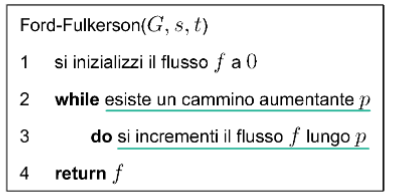
\includegraphics[width=0.5\linewidth]{Images/reti_di_flusso/ford_fulkerson.png}
\end{figure}
Definiamo come \textbf{capacità residua} la quantità di flusso netto addizionale che possiamo inviare su di un certo acro prima di saturarlo. Questa si calcola nel seguente modo:
\[c_f(u, v) = c(u, v) - f(u, v)\]
Quando il flusso netto $f(u, v)$ è negativo, allora vuol dire che la capacità residua $c_f(u,v)$ è maggiore rispetto alla capacità $c(u, v)$. Questo ci viene utile nel momento in cui l'algoritmo deve capire quanto può eliminare in termini di flusso da quell'arco.
Chiamiamo \textbf{rete residua} di $G$ indotta da $f$ la rete $G_f=(V,E_f)$ dove:
\[E_f=\{(u,v) \in V \times V: c_f(u,v)>0\}\]
Ogni arco nella rete è, quindi, chiamato \textbf{arco residuo} e questo può ammettere flusso netto strettamente positivo.Questi archi possono provenire da due fonti:
\begin{itemize}
    \item $E$ (Archi originali): I tubi veri che hanno ancora spazio vuoto;
    \item $E^T$ (Archi trasposti/inversi): I tubi dai quali è possibile togliere il flusso.
\end{itemize}
Vale che $|E_f| \leq 2E$. 
Data una rete di flusso, un \textbf{cammino aumentate }$p$ è un cammino semplice dalla sorgente al pozzo nella rete residua $G_f$. Per definizione di rete residua, ogni arco $(u, v)$ su un cammino aumentante ammette un flusso netto positivo addizionale senza violare il vincolo di capacità dell'arco. 
\subsection*{Lemma 2}
Sia $(G,c)$ una rete di flusso e sia $f$ un flusso di G e sia $p$ un cammino aumentante in $G_f$. Si definisca una funzione $f_p: V \times V \to R$ come:
\[
f_p(u, v) = 
\begin{cases} 
   c_f(p) & \text{se } (u, v) \text{ è su } p \\
   -c_f(p) & \text{se } (v, u) \text{ è su } p \\
   0 & \text{altrimenti}
\end{cases}
\]
Dimostriamo che $f_p$ è un flusso in $G_f$:
\begin{itemize}
    \item \textbf{Vincolo di Capacità}: Consideriamo i due casi:
    \begin{itemize}
        \item Se $f_p(u,v)\leq 0$, allora $f_p \leq c_f(u,v)$ per definizione dato che $c_f$ non può essere negativo e, inoltre, vuol dire che quell'arco non appartiene al cammino aumentante.
        \item Se $f_p(u,v) > 0$, allora $(u,v)$ fa parte del cammino aumentante e, quindi, il vincolo è banalmente rispettato poiché: 
        \[f_p(u,v) = c_f(p) = \min \{ c_f(u',v') \mid (u',v') \in p \} \le c_f(u,v)\]
    \end{itemize}
    \item \textbf{Antisimmetria}: Dobbiamo verificare che $f_p(u,v) = -f_p(v,u)$ per ogni $(u,v) \in V \times V$. Dunque:
    \begin{itemize}
        \item Se $f_p(u,v) = 0$:
        Significa che $(u,v) \notin p$ e $(v,u) \notin p$. Di conseguenza anche $f_p(v,u) = 0$.
        \[ 0 = -0 \quad \checkmark \]

        \item Se $f_p(u,v) \ne 0$:
        Allora uno dei due archi appartiene al cammino $p$.
        \begin{itemize}
            \item Caso $(u,v) \in p$:
            \[ f_p(u,v) = c_f(p) \quad \text{e} \quad f_p(v,u) = -c_f(p) \]
            \[ \Rightarrow f_p(u,v) = -f_p(v,u) \]
            
            \item Caso $(v,u) \in p$:
            \[ f_p(v,u) = c_f(p) \quad \text{e} \quad f_p(u,v) = -c_f(p) \]
            \[ \Rightarrow f_p(u,v) = -f_p(v,u) \]
        \end{itemize}
    \end{itemize}
    \item \textbf{Conservazione}: Dobbiamo verificare che per ogni nodo intermedio $u \in V \setminus \{s,t\}$, il flusso netto uscente è nullo: $\sum_{v \in V} f_p(u,v) = 0$.

    Analizziamo due casi per il nodo $u$:

    \begin{itemize}
        \item \textbf{Caso $u \notin p$ (il nodo non è sul cammino):}
        Per ogni $v \in V$, né $(u,v)$ né $(v,u)$ sono su $p$.
        Quindi $f_p(u,v) = 0$ per ogni $v$.
        \[ \sum_{v \in V} f_p(u,v) = 0 \]

        \item \textbf{Caso $u \in p$ (il nodo è sul cammino):}
        Poiché $u$ è un nodo interno del cammino semplice $p$, esiste un unico vertice $v'$ che precede $u$ e un unico vertice $v''$ che segue $u$ nel cammino ($v' \to u \to v''$).
        
        I valori del flusso sono:
        \begin{align*}
            v = v'' & \implies f_p(u,v'') = c_f(p) \quad (\text{flusso in avanti}) \\
            v = v'  & \implies f_p(u,v') = -c_f(p) \quad (\text{flusso all'indietro verso il predecessore}) \\
            v \notin \{v', v''\} & \implies f_p(u,v) = 0
        \end{align*}
        
        Facendo la somma totale:
        \[ \sum_{v \in V} f_p(u,v) = c_f(p) - c_f(p) + 0 = 0 \]
    \end{itemize}
\end{itemize}
\subsection*{Lemma 3}
Sia $(G,c)$ una rete di flusso e sia $f$ un flusso di $G$. Sia $G_f$ la rete residua di $G$ indotta da $f$ e sia $f'$ un flusso in $G_f$, allora la somma $f+f'$ è un flusso in $G$ con valore $|f+f'| = |f| + |f'|$. Cioè, Se hai un flusso esistente ($f$) e trovi un flusso aggiuntivo ($f'$) nella rete residua, puoi sommarli matematicamente e il risultato sarà ancora un flusso valido per la rete originale, ma più grande. 
Dimostriamo che è un flusso:
\begin{itemize}
    \item \textbf{Antisimmetrica}:Sappiamo che, per definizione, $(f+f')(u, v) = f(u,v)+f'(u,v)$. Dunque vediamo che:
    \[f(u,v) + f'(u,v) = -f(v,u)-f'(v,u) = -(f(v,u)+f'(v,u)) = -(f+f')(v,u)\]
    Cioè la proprietà è rispettata.
    \item \textbf{Vincolo di capacità}: Dobbiamo essere sicuri che sommando flussi non scoppino i tubi (non superiamo $c(u,v)$). Vediamo che:
    \begin{align*}
        (f+f')(u,v) = f(u, v) + f'(u, v) \leq f(u,v) +c_f(u,v)\\
        &\leq f(u,v) + (c(u,v)- f(u,v))  = c(u, v)
    \end{align*}
    \item \textbf{Conservazione del flusso}: Sappiamo che, per definizione:
    \begin{align*}
        \sum_{v\in V} (f+f')(u, v) = \sum_{v \in V} (f(u,v)+ f'(u,v))\\
        & = \sum_{v \in V} f(u, v) + \sum_{v \in V} f'(u,v) = 0+0 = 0
    \end{align*}
\end{itemize}


Dunque, sia $(G,c)$ una rete di flusso e sia $f$ un flusso di G, sia $p$ un cammino aumentante in $G_f$. Sia $f_p$ il flusso in $G_f$ definito come nel lemma 3 e sia $f': V \times V \to R$ la funzione:
\[f' = f +f_p\]
Allora $f'$ è un flusso in G con valore $|f'| = |f| + |f_p|> |f|$. Scriveremo dunque la procedura Ford Fulkerson come segue:
\begin{figure}[H]
    \centering
    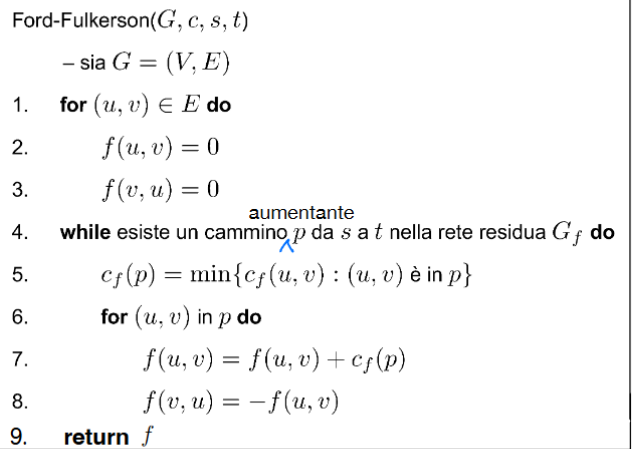
\includegraphics[width=0.5\linewidth]{Images/reti_di_flusso/ff_2.png}
\end{figure}

Analizziamo il tempo di esecuzione della procedura:
\begin{itemize}
    \item Per il ciclo all'inizio, abbiamo un tempo $O(E)$.
    \item Per il ciclo while da 4 a 8, questo può essere eseguito un massimo di $|f^*|$ poiché il valore del flusso aumenta almeno di una unità ogni iterazione. Un cammino aumentante a ogni iterazione può essere calcolato in tempo $O(E)$
\end{itemize}
La procedura ha un tempo di esecuzione pari a $O(E|f^*|)$ dove $f^*$ è il flusso massimo trovato dall'algoritmo. È importante notare che l'algoritmo potrebbe non terminare in caso di numeri non razionali.\footnote{C'è un pdf che mostra un esempio di questa casistica che non ho inserito.} Si noti che è possibile, scegliendo il cammino aumentate p con una visita in ampiezza, migliorare la complessità temporale a $O(VE^2)$. Questa variante si chiama \textbf{Algoritmo di Edmonds-Karp} e non ha problemi in caso di esecuzione con numeri irrazionali. 
\section{Tagli in Reti di flusso}
Definiamo un \textbf{Taglio (S, T)} in una rete di flusso $(G,c)$ con sorgente s e posso t una partizione di V in S e $T = V-S$ tale che $s \in S$ e $t \in T$. 
Se f è un flusso, allora il \textbf{flusso netto attraverso il taglio $(S,T)$} è definito come:
\[f(S,T) = \sum_{u \in S, v \in T}f(u, v)\]
La \textbf{capacità del taglio} è:
\[c(S,T) = \sum_{u \in S, v \in T}c(u, v)\]
\subsection*{Lemma 4}
Sia $f$ un flusso su una rete con sorgente s e pozzo t, e sia $(S,T)$ un taglio. Allora il flusso netto attraverso $(S,T)$ è $f(S,T)= |f|$. 
Si dimostra banalmente poiché:
\begin{align*}
    f(S,T) = f(S,V) - f(S,S) \quad \text{ Consideriamo che $f(S,S) = 0$}\\
    = f(S,V) = f(s,V)+f(S-s,V) \quad \text{ $f(S-s,V) = 0$ poiché sono nodi intermedi}\\
    =|f|
\end{align*}

Ne segue che il valore di un qualunque flusso $f$ in una rete di flusso è limitato superiormente dalla capacità di un qualunque taglio di G. Si può dimostrare come segue:\footnote{Ciao Angelo, io non so se stai leggendo questa cosa, tuttavia se lo stai facendo sappi che sto imprecando mentalmente. P.S.: Palle}
\begin{align*}
    |f| = f(S,T)\\
    & = \sum_{u \in S, v \in T} f(u,v) \\
    &\leq \sum_{u \in S, v \in T} c(u,v) = c(S, T)
\end{align*}
Ne segue che $sup (|f|) \leq \min c(S, T)$. Da qui ne possiamo derivare il teorema che segue.
\section{Teorema del Massimo Flusso/Minimo Taglio}
Sia $f^*$ un flusso in una rete di flusso con sorgente s e pozzo t, allora abbiamo che le seguenti proprietà sono equivalenti:\footnote{Cioè, se ne vale una valgono tutte.}
\begin{itemize}
    \item $|f^*|$ è un flusso massimo in G.
    \item La rete residua $G_{f^*}$ non contiene alcun cammino aumentante.
    \item $|f^*| = c(S^*, T^*)$ per qualche taglio di G.
\end{itemize}
Ne segue che il massimo flusso $|f|$ è uguale al minimo $c(S,T)$. Che vuol dire che la massima quantità di acqua che puoi spingere da $A$ a $B$ è esattamente uguale alla capacità del collo di bottiglia' più stretto della rete.

\subsection*{1. $(1 \implies 2)$ (Per assurdo)}
Supponiamo per assurdo che $f^*$ sia massimo ma che esista un cammino aumentante $p$ in $G_{f^*}$.
\begin{itemize}
    \item Possiamo aumentare il flusso lungo $p$ di una quantità $f_p > 0$.
    \item Il nuovo flusso sarà $f' = f^* + f_p$.
    \item Il valore del nuovo flusso è $|f'| = |f^*| + |f_p| > |f^*|$.
\end{itemize}
Questo contraddice l'ipotesi che $f^*$ fosse massimo.

\subsection*{2. $(2 \implies 3)$ (Costruttiva)}
Supponiamo che non esistano cammini aumentanti da $s$ a $t$ in $G_{f^*}$.
Costruiamo l'insieme $S^*$ dei nodi raggiungibili da $s$ nella rete residua:
\[ S^* = \{ v \in V \mid \text{esiste un cammino } s \to v \text{ in } G_{f^*} \} \]
Poniamo $T^* = V \setminus S^*$.
\begin{itemize}
    \item Poiché $t$ non è raggiungibile, $t \in T^*$, quindi $(S^*, T^*)$ è un taglio valido.
    \item Per ogni arco $(u, v)$ con $u \in S^*$ e $v \in T^*$, deve valere $f(u, v) = c(u, v)$ (l'arco è saturo), altrimenti $(u, v)$ esisterebbe nella rete residua e $v$ sarebbe in $S^*$.
    \item Di conseguenza, il flusso netto attraverso il taglio eguaglia la capacità:
    \[ |f^*| = f(S^*, T^*) = \sum_{u \in S^*, v \in T^*} c(u, v) = c(S^*, T^*) \]
\end{itemize}

\subsection*{3. $(3 \implies 1)$ (Deduzione diretta)}
Supponiamo che $|f^*| = c(S^*, T^*)$.
Per il corollario della dualità debole, sappiamo che per \textit{qualsiasi} flusso $f$ e \textit{qualsiasi} taglio $(S, T)$ vale sempre:
\[ |f| \le c(S, T) \]
In particolare:
\[ |f| \le c(S^*, T^*) = |f^*| \]
Poiché nessun flusso può superare questo valore, $f^*$ deve essere necessariamente un flusso massimo. 
